\begin{figure}[H]
\center

\includegraphics[width=0.2\textwidth]{elasticsearch.png}
\label{fig:elasticsearchlogo.png}
\end{figure}
%\begin{wrapfigure}{r}{0.25\textwidth}
%\begin{center}
%
\includegraphics[width=0.25\textwidth]{elasticsearch.png}
%\end{center}
%\caption{A gull}
%\end{wrapfigure}
\section{Présentation de Elasticsearch}
Elasticsearch est moteur de recherche et d'analyse en temps réel. Il permet l'exploration
de données de façon très rapide par des recherches, que ce soit par des recherches
\gls{fulltext}, ou bien des recherches structurées.

Elasticsearch est depuis peu développé par la société \emph{Elastic}. C'était, à 
la base, un projet du développeur Shay Banon, qui souhaitait concevoir une API simplifié
pour la bibliothèque de moteur de recherche : Apache Lucene\fnu[Page du projet Lucene ]{https://lucenenet.apache.org/}.

Elasticsearch et la stack ELK est en passe de devenir un standard dans l'industrie.
En effet le logiciel à une utilisation assez versatile, de l'aide à la prise de 
décision en temps réelle à l'analyse de code source. Et à l'heure actuelle, la capacité 
à exploiter les masses de données et de méta données accumulées chaque jour devient 
un enjeu économique majeur (mais pas seulement \ldots). Enfin l'un des principaux 
atouts d'Elasticsearch réside dans son aptitude à pouvoir passer à l'échelle simplement.

\section{Installation}
Avant même de regarder les différentes dépendances nécessaires à l'utilisation de
Elasticsearch il est recommandé de vérifier que l'on utilise bien la même version
que son compère logstash (vérifier la documentation).

Son installation est sensiblement la même que son comparse logstash puisque ce logiciel 
nécessite également l'installation des dépendances \emph{jruby} et \emph{openjdk-7-jre}
à noter qu'il fonctionne également sur openjdk-8-jre.

Là aussi les paquets debian officiels n'existant pas on utilisera celui fourni par 
elastic.co\footnote{https://download.elastic.co/elasticsearch/elasticsearch/elasticsearch-1.5.1.deb}.
Et ici aussi le paquet est un peu approximatif puisqu'il faut rajouter certains chemin, et ajouter des droits.




Acompleter et revoir
p24-26
 test


\section{Sense}
Sense est un module chrome développé par Boaz Leskes, il sert de front-end à ElasticSearch.
Le développement (public) de ce module est maintenant arrêté. Il fait parti de 
\emph{Marvel} le logiciel de monitoring et d'optimisation, vendu\footnote{voir bas 
de page : \url{https://www.elastic.co/products/marvel/signup.html}} 
par la société \emph{elastic}.


\subsection{Installation}
Installer ce logiciel est simple comme installer une extension Chrome\footnote{testé sur chromium}
tierce.
Tout d'abord : récupérer le module à l'adresse \url{https://github.com/bleskes/sense}
en utilisant par exemple : 
\begin{lstlisting}[style=code,label=lst:gitclonesense]
git clone https://github.com/bleskes/sense.git
\end{lstlisting}

Il suffit ensuite de l'activer dans chromium :\\ 
chrome://extension => Developer mode => Load unpacked extension.

\begin{figure}[H]
\center
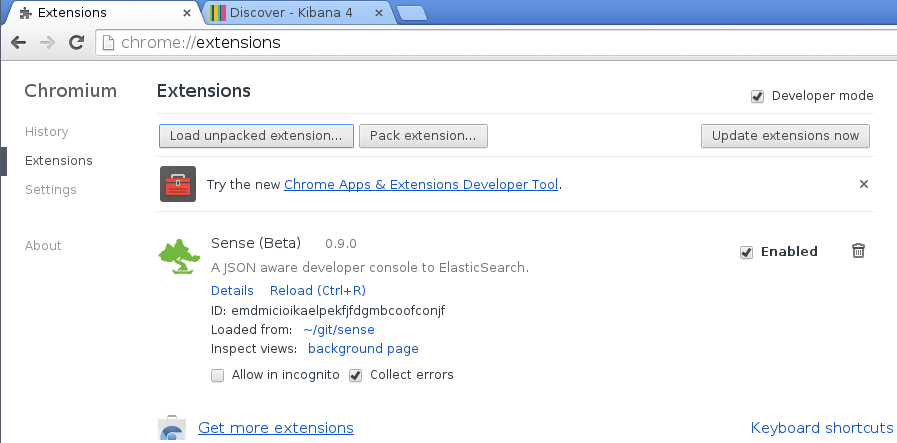
\includegraphics[width=15cm]{senseinstall.png}
\label{fig:senseinstall}
\caption{Plugin Sense installé dans chromium}
\end{figure}

Et voilà ! \footnotesize{(avec un accent anglais)}

\subsection{Utilisation de Sense}
L'utilisation de Sense est assez simple via son interface :

\begin{figure}[H]
\center
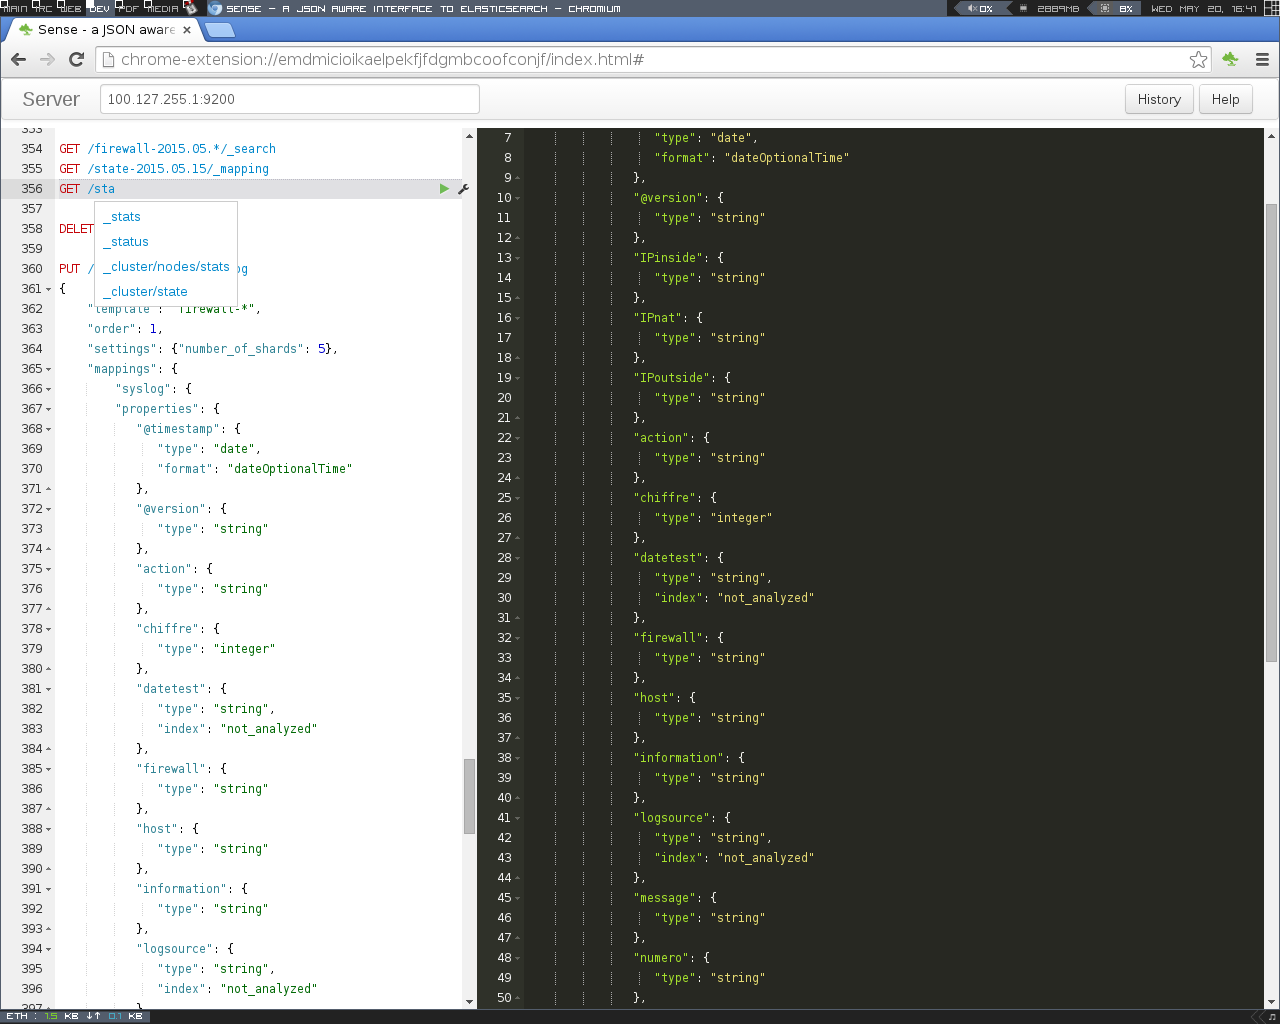
\includegraphics[width=15cm]{sensegui.png}
\label{fig:sensegui.png}
\caption{Vue générale de Sense}
\end{figure}

La difficulté se situe évidemment plutôt du coté de l'appréhension, la configuration
et l'optimisation de Elasticsearch.

Nous allons avec l'image ci-dessous \ref{fig:sensegui2.png} brièvement expliquer le fonctionnement de Sense
\begin{figure}[H]
\center
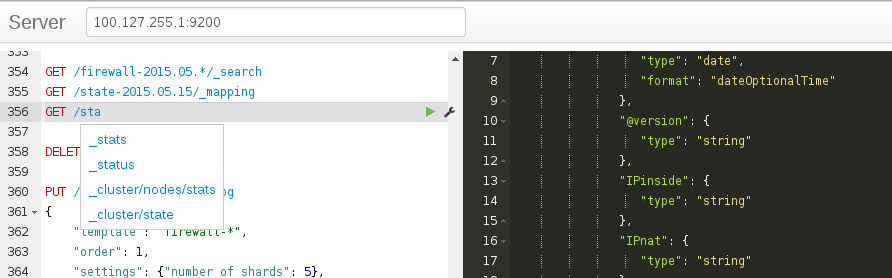
\includegraphics[width=15cm]{sensegui2.png}
\label{fig:sensegui2.png}
\caption{Zoom sur les fonctionnalités de Sense}
\end{figure}
Le formulaire \textbf{Server} situé en haut correspond à l'adresse et au port d'écoute 
de l'instance Elasticsearch sur laquelle on souhaite travailler.

Le panneau de gauche correspond au \textbf{panneau de requêtes}. On utilise l'api REST d'elasticsearch
pour envoyer des requêtes (recherches, modification etc, point sur l'API prévu 
ultérieurement). Il est à noté que le panneau de gauche est doté d'une autocomplétion
pour les fonctions et configurations standards dans elasticsearch.

Le panneau de droite est le \textbf{panneau de réponse} aux requêtes.


